\documentclass[11.5pt]{sig-alternate} % sets document style to sig-alternate
% packages
% typesetting
% \usepackage{dirtytalk} % can be used to typset quotes easier, automatically sets correct quotation marks with \say{content}
% \usepackage{hanging} % hanging paragraphs with \hanging, like in references. doesn't translate to HTML
\usepackage[defaultlines=3,all]{nowidow} % avoid widows
\usepackage[pdfpagelabels=false]{hyperref} % produce hypertext links, includes backref and nameref
\usepackage{xurl} % defines url linebreaks, loads url package
\usepackage{microtype} % better typography
\usepackage{ragged2e}
% \usepackage{textcomp} % for better tildes
% \newcommand{\texttildemid}{\raisebox{0.4ex}{\texttildelow}}
% layout
\usepackage{calc} % so we can do inline math within \setlength
% \usepackage{enumitem} % control layout of itemize, enumerate, description
\usepackage{fancyhdr} % control page headers and footers
% \usepackage{float} % improved interface for floating objects, adds H float
% \usepackage{multicol} % intermix single and multiple column pages
% \textgreek % typeset greek letters in text mode
% language
\usepackage[utf8]{inputenc} % utf8 encoding, wider character set
\usepackage[english]{babel} % multilanguage support
% misc
\usepackage{graphicx} % builds upon graphics package, \includegraphics
%\usepackage{lastpage} % reference number of pages
\usepackage{xcolor} % color extensions
\usepackage[backend=biber, style=apa]{biblatex} % sophisticated bibliographies % necessary for HTML to display author info and date on abstract page
\usepackage{csquotes} % advanced quotations, makes biblatex happy
\usepackage{authblk} % support for footnote style author/affiliation
% tables and figures
%\usepackage{array} % extend array and tabular environments
\usepackage{caption} % customize captions in figures and tables (rotating captions, sideways captions, etc)
%\usepackage{cuted} % allow mixing of \onecolumn and \twocolumn on same page
\usepackage{multirow} % create tabular cells spanning multiple rows
%\usepackage{subfigure} % deprecated, support for manipulation of small figures
\usepackage{tabularray} % better table construction, does not translate to HTML
%\usepackage{wrapfig} % allows figures or tables to have text wrapped around them
% dummy text
%\usepackage{blindtext} % blind text dummy text
%\usepackage{kantlipsum} % Kant style dummy text
\usepackage{lipsum} % lorem ipsum dummy text

\pagestyle{fancy} % sets pagestyle to fancy for fancy headers and footers
% allows the header to take the full width of the page https://www.reddit.com/r/LaTeX/comments/awtrb2/how_to_you_make_the_headerfooter_extend_the/
\newlength{\oddmarginwidth}
\setlength{\oddmarginwidth}{1in+\hoffset+\oddsidemargin}
\newlength{\evenmarginwidth}
\setlength{\evenmarginwidth}{\evensidemargin+1in}
\fancyhfoffset[LO,RE]{\oddmarginwidth}
\fancyhfoffset[LE,RO]{\evenmarginwidth}

% header and footer
% modern way to set header image
\renewcommand{\headrulewidth}{0pt} % defines thickness of line under header
\renewcommand{\footrulewidth}{0pt} % defines thickness of line above header
\setlength\headheight{80.0pt} % sets height between top margin and header image, effectively moves page contents down
\addtolength{\textheight}{-80.0pt} % seems to affect the lower height. maybe only works properly if footer numbers enabled?
\fancyhf{}
\fancyhead[CE, CO]{
\includegraphics[width=\pdfpagewidth]{headerImage.png}}

\hypersetup{colorlinks=true,urlcolor=blue} % sets link color to blue
\urlstyle{same} % sets url typeface to same as rest of text

% set caption and figure to italics, label bold, left align captions, does not transfer to HTML
\captionsetup{labelfont=bf, font={large, it}, justification=raggedright, singlelinecheck=false}
\renewcommand\theContinuedFloat{\alph{ContinuedFloat}} % has something to do with subfigures... don't remember why i used it

%this next bit is confusing, but essentially changes the width of the abstract. Seems to have been copied from this https://tex.stackexchange.com/questions/151583/how-to-adjust-the-width-of-abstract
\let\oldabstract\abstract
\let\oldendabstract\endabstract
\makeatletter %changes @ catcode to enable modification (in parsep)
\renewenvironment{abstract} %alters the abstract environment
{\renewenvironment{quotation}%
               {\list{}{\addtolength{\leftmargin}{1em} % change this value to add or remove length to the the default ?
                        \listparindent 1.5em%
                        \itemindent    \listparindent%
                        \rightmargin   \leftmargin%
                        \parsep        \z@ \@plus\p@}%
                \item\relax}%
               {\endlist}%
\oldabstract}
{\oldendabstract}
\makeatother %changes @ catcode to disable modification

% checks
% italics 
% links
% dashes
% tildes
\begin{document}
\title{Evaluation of a Guide to Accessing Accommodations During Medical School Created by and for Students with Disabilities}

\author[1]{\large \color{blue} Nora Newcomb} % make sure there are no spaces after the author's name
\author[1]{\large \color{blue} Emily Coughlin}
\author[2]{\large \color{blue} Zainub Dhanani}
\author[3]{\large \color{blue} Kie Fujii}
\author[4]{\large \color{blue} Lily Upp}
\author[5]{\large \color{blue} Harika Kottakota}
\author[1]{\large \color{blue} Rahul Mhaskar}
\author[1]{\large \color{blue} Andrew Galligan}

\affil[1]{University of South Florida Health Morsani College of Medicine}
\affil[2]{Stanford University School of Medicine}
\affil[3]{Hackensack Meridian School of Medicine}
\affil[4]{The University of Chicago Pritzker School of Medicine}
\affil[5]{David Geffen School of Medicine at UCLA}
\toappear{} % the sig.alternate document type includes a copyright warning that appears at the bottom of the first page. This makes that not appear/be empty. Don't ask my why it's there in the first place /shrug

\maketitle % prints article title
\begin{@twocolumnfalse} 
\begin{abstract}
\item %the abstract is a quotation and a list, so this must be an item
\begin{large}
\textit{Medical students with disabilities constitute 7.6\% of allopathic (MD) and 4.3\% of osteopathic (DO) programs, and they are entitled to reasonable accommodation, per the Americans with Disabilities Act. However, research has demonstrated that disabled medical students often encounter barriers when accessing accommodations. In response to these barriers, Medical Students with Chronic Illness and Disability (MSDCI) National created the MSDCI Guide to Accessing Disability Accommodations During Undergraduate Medical Education (the Guide). We conducted a program evaluation to evaluate the efficacy of the Guide as a resource to the members of MSDCI, a program evaluation was conducted. A Qualtrics survey was distributed though the MSDCI listserv, and 29 complete responses were received. Responses were analyzed with descriptive statistics. All respondents agreed or strongly agreed with the statement “I would recommend this guide to other medical students with disability and/or chronic illness.” The sections rated “most useful” were “Accessing USMLE Accommodations” and “Understanding Materials for Accommodation.” The section rated “least useful” was “Accessing CASPer Accommodations.” Freeform comments highlighted a need for greater inclusion of DO-specific topics, and a more detailed explanation of the rights of disabled medical students. This feedback demonstrates that the Guide is a good resource for the disabled and chronically ill medical students in the MSDCI community. Future editions of the Guide will include more DO-related topics and exclude pre-medical topics.}
\item Keywords: disability, medical education, access, accommodations
\end{large}     
\end{abstract}
\end{@twocolumnfalse}

%% AUTHOR INFORMATION
\textbf{*Corresponding Author, Nora Newcomb}\\ % corresponding author
\href{mailto:ndnewcomb@usf.edu}{(ndnewcomb@usf.edu)} \\ % author email
\textit{Submitted Nov 4 2023} \\ % submitted date
\textit{Accepted Aug 29 2024} \\ % accepted date
\textit{Published Online Jan 17 2025} \\ %published online date, updated after author approval
\textit{DOI: 10.14448/jsesd.16.0004} \\ % doi, updated after author approval, in spreadsheet on server
\pagebreak 
\clearpage % both needed to go to next page
\begin{large}

\section*{INTRODUCTION}
Medical students with disabilities constitute 7.6\% of allopathic (MD) and 4.3\% of osteopathic (DO) programs (Meeks et al., 2021; Meeks et al., 2020). As per Section 504 of the Rehabilitation Act of 1973 (Section 504) and the Americans with Disabilities Act of 1990 and 2008 (ADA), these students must be provided reasonable accommodations throughout their education (Office of Civil Rights, 2023; “ADA Amendments,” 2008). However, research demonstrates that disabled medical students often encounter barriers when in accessing or implementing those accommodations, including complex administrative policies, lack of qualified Disability Service Providers (DSPs), and social factors such as stigma and discrimination (Meeks \& Jain, 2018; Meeks \& Jain, 2016).
\\
\subsection*{Rationale of current study}
To address barriers to accessing disability accommodations in medical school, also known as undergraduate medical education (UME), the authors created the “MSDCI Guide to Accessing Disability Accommodations During Undergraduate Medical Education (the Guide).” The Guide was developed to be a comprehensive resource, with the primary objectives of educating medical students with disabilities on their rights as well as the process of receiving reasonable accommodations (Newcomb \& Upp (Eds.), 2022). This study aims to evaluate the usefulness of the Guide.

\section*{METHODS}
\subsection*{Guide Development}
Medical Students with Disability and Chronic Illness National (MSDCI) is a national student-led organization dedicated to community, advocacy, education, and accessibility. MSDCI shapes its efforts around the needs of its membership. There was call from the member body for a guide to accommodations, given the complicated policies and processes around accommodations access in medical education. Development of the Guide began in the Spring of 2021. Topic selection was crowdsourced through informal input from members with relevant lived experience.  Writers were recruited from within the MSDCI community. The two main editors (NN, LU) were responsible for reviewing all sections for content, clarity and continuity. 

\begin{figure*}[htbp]
    \centering
    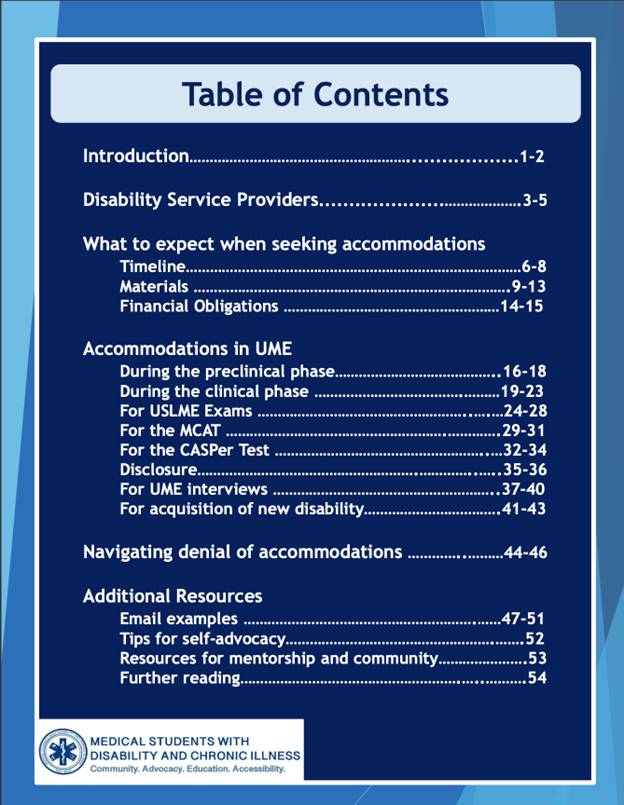
\includegraphics[width=0.9\textwidth]{images/fig1.png}
    \caption{Table of Contents for the Guide}
    \label{Figure 1}
    \justifying
    \textit{Note}. Reprinted from Newcomb, N  \&  Upp, L. (Eds.). (2022). \textit{MDSCI Guide to Accessing Disability Accommodations During Undergraduate Medical Education}. msdci.org. Reprinted with permission.
\end{figure*}

Efforts were made to ensure that the information included was legible (fig. 2), to accommodate those with low vision, learning disabilities and other related disabilities. The Guide was organized to facilitate general ease of use and localization of relevant information.

\begin{figure*}[htbp]
    \centering
    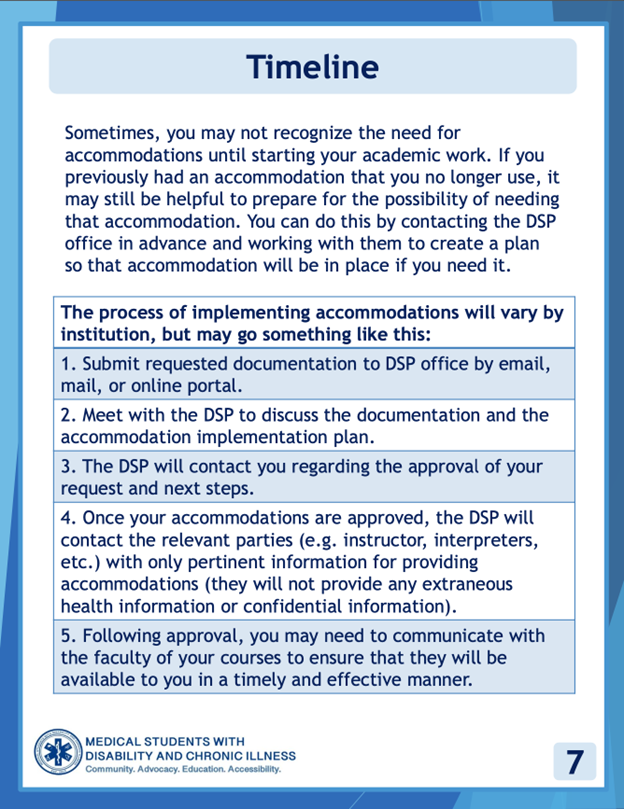
\includegraphics[width=0.9\textwidth]{images/fig2.png}
    \caption{Excerpt of the Guide Demonstrating Layout}
    \label{Figure 2}
    \justifying
    \textit{Note}. Reprinted from Newcomb, N  \&  Upp, L. (Eds.). (2022). \textit{MDSCI Guide to Accessing Disability Accommodations During Undergraduate Medical Education}. msdci.org. Reprinted with permission.
\end{figure*}

Additionally, the Guide includes usable tools, such as email templates and guidelines for keeping email information confidential (fig. 3).

\begin{figure*}[htbp]
    \centering
    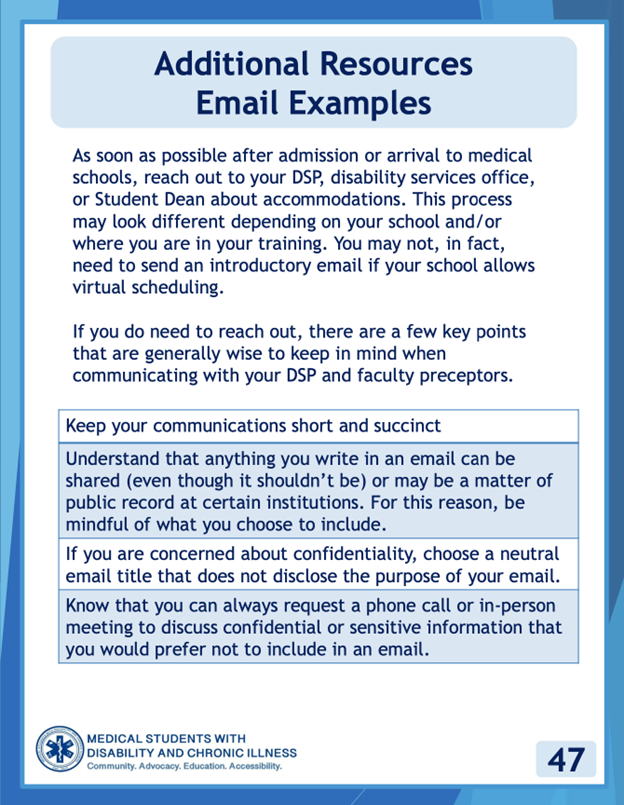
\includegraphics[width=0.9\textwidth]{images/fig3.png}
    \caption{Advice on Emailing a Disability Service Provider (DSP)}
    \label{Figure 3}
    \justifying
    \textit{Note}. Reprinted from Newcomb, N  \&  Upp, L. (Eds.). (2022). \textit{MDSCI Guide to Accessing Disability Accommodations During Undergraduate Medical Education}. msdci.org. Reprinted with permission.
\end{figure*}

The Guide was posted to the MSDCI website in February 2022. It was further distributed via the MSDCI listserv, through MSDCI social media, networks of local MSDCI chapters and the AAMC student representative network. 

To evaluate the Guide, the researchers developed a 12-question survey that addressed 1) the demographics of participants and their training programs, 2) the efficacy of The Guide’s 18 sections in increasing knowledge via a 4-point scale (1=did not increase, 4=strongly increased), and 3) suggested improvements to the guide via free response questions. The anonymous survey link was emailed to MSDCI’s members and the 19 existing institutional chapters, posted on MSDCI’s social media platforms and distributed to attendees at Disability Advocacy Coalition in Medicine's 2022 Interprofessional Conference.  The survey was open from September 8, 2022 to October 15, 2022. All survey responses were anonymous. Participants were offered the option to be entered in a drawing for one of ten \$5 gift cards.

Data were analyzed by descriptive statistics and are presented as frequencies and proportions. Participants who indicated they did not read a given section of the guide were excluded from its analysis. Participants who indicated they did not read any portion of the guide and did not provide a reason were excluded from the analysis entirely.

\subsection*{Institutional Review Board (IRB) Approval}

Under the IRB compliance office guidelines set by the University of South Florida Health Morsani College of Medicine, this survey falls under the designation of program evaluation and therefore does not require IRB approval.

\section*{Results}
The survey received 29 valid responses. Respondents hailed from twelve different states and representing all years of training. When asked how they were made aware of the Guide, with an option to select multiple options, 13 (44.8\%) respondents indicated that they learned about the Guide through the MSDCI listserv, 4 (13.8\%) said it was through the MSDCI website, 3 (10.3\%) indicated that it was through their institutional chapter, 3 (10.3\%) said it was through a fellow student, 2 (6.9\%) from the DAC Med 2022 Conference and 1 (3.4\%) from MSDCI’s social media presence. Respondents had a wide range of disabilities, the most common being 10 (34.5\%) people identifying as having a chronic illness/invisible disability (Table 1).

\begin{table}[ht]
\caption{Demographics}
\begin{tabular}{|l|l|}
\hline
Question & N(\%) \\ \hline
\begin{tabular}[x]{@{}l@{}} \textbf{What type of medical training program are you enrolled in?} \\ \textit{DO/Osteopathic} \\ \textit{MD/Allopathic} \\ \textit{MD/PhD} \end{tabular} & \begin{tabular}[x]{@{}l@{}} \\ 4 (13.8) \\ 23 (79.3) \\ 2 (6.9) \end{tabular} \\ \hline
\begin{tabular}[x]{@{}l@{}} \textbf{What year in training are you?} \\ \textit{MS1/OMS1} \\ \textit{MS2/OMS2} \\ \textit{MS3/OMS3} \\ \textit{MS4/OMS4} \\ \textit{Other (research year, leave, etc.)} \end{tabular} & \begin{tabular}[x]{@{}l@{}} 7 (24.1) \\ 8 (27.6) \\ 8 (27.6) \\ 3 (10.3) \\ 3 (10.3) \end{tabular} \\ \hline
\begin{tabular}[x]{@{}l@{}} \textbf{Do you identify as a person with a disability and/or chronic illness?} \\ \textit{No} \\ \textit{Yes} \end{tabular} & \begin{tabular}[x]{@{}l@{}} \\ 7 (24.1) \\ 22 (75.9) \end{tabular} \\ \hline
\begin{tabular}[x]{@{}l@{}} \textbf{If you answered “yes” to the previous question, please indicate the category to which your disability and/or chronic illness best fits (select all that apply)} \\ \textit{Chronic Illness/Invisible}  \\ \textit{Mental health/Psychiatric}  \\ \textit{Intellectual} \\ \textit{Learning} \\ \textit{Neurodivergence} \\ \textit{Neurological} \\ \textit{Physical} \\ \textit{Sensory (hearing)} \\ \textit{Sensory (vision)} \end{tabular} & \begin{tabular}[x]{@{}l@{}} \\ 10 (34.5) \\ 4 (13.8) \\ 1 (3.4) \\ 3 (10.3) \\ 4 (13.8) \\ 4 (13.8) \\ 5 (17.2) \\ 2 (6.9) \\ 2 (6.9) \end{tabular} \\ \hline
\end{tabular}
\end{table}

\begin{table*}[htp]
\caption{Knowledge and Effectiveness of Each Section}
\begin{tabular}{|l|l|l|l|l|l|l|}
\hline
& \multicolumn{3}{|l|}{Knowledge, N (\%)} & \multicolumn{3}{|l|}{Effectiveness, N (\%)} \\ \hline
& Did not increase & Increased & Strongly increased & Moderately ineffective & Moderately effective & Very effective \\ \hline
Identifying a Disability Service Provider & 2 (6.9) & 10 (34.5) & 1 (3.4) & 0 (0) & 4 (13.8) & 8 (27.6) \\ \hline
Understanding Timelines for Accommodations & 0 (0) & 15 (51.7) & 3 (10.3) & 0 (0) & 6 (20.7) & 8 (27.6) \\ \hline
Understanding Materials for Accommodations & 1 (3.4) & 14 (48.3) & 3 (10.3) & 0 (0) & 6 (20.7) & 7 (24.1) \\ \hline
Understanding Financial Obligations for Accommodations & 1 (3.4) & 10 (34.5) & 2 (6.9) & 0 (0) & 4 (13.8) & 5 (17.2) \\ \hline
Accessing Preclinical Accommodations & 1 (3.4) & 11 (37.9) & 1 (3.4) & 1 (3.4) & 3 (10.3) & 3 (10.3) \\ \hline
Accessing Clinical Accommodations & 2 (6.9) & 10 (34.5) & 2 (6.9) & 1 (3.4) & 5 (17.2) & 3 (10.3) \\ \hline
Accessing USMLE\textsuperscript{1} Accommodations & 1 (3.4) & 12 (41.4) & 3 (10.3) & 0 (0) & 7 (24.1) & 5 (17.2) \\ \hline
Accessing MCAT\textsuperscript{2} Accommodations & 1 (3.4) & 6 (20.7) & 1 (3.4) & 0 (0) & 3 (10.3) & 1 (3.4) \\ \hline
Accessing CASPer\textsuperscript{3} Accommodations & 0 (0) & 8 (27.6) & 1 (3.4) & 1 (3.4) & 2 (6.9) & 1 (3.4) \\ \hline
Navigating Disclosure & 0 (0) & 12 (41.4) & 2 (6.9) & 0 (0) & 5 (17.2) & 3 (10.3) \\ \hline
Accommodations for UME Interviews & 0 (0) & 7 (24.1) & 1 (3.4) & 0 (0) & 3 (10.3) & 1 (3.4) \\ \hline
Accessing Accommodations for a Newly Acquired Disability & 1 (3.4) & 8 (27.6) & 1 (3.4) & 0 (0) & 4 (13.8) & 2 (6.9) \\ \hline
Navigating Denial of Accommodations & 0 (0) & 10 (34.5) & 1 (3.4) & 0 (0) & 4 (13.8) & 2 (6.9) \\ \hline
Email Examples/Templates & 0 (0) & 9 (31.0) & 4 (13.8) & 0 (0) & 5 (17.2) & 6 (20.7) \\ \hline
Tips for Self-Advocacy & 1 (3.4) & 12 (41.4) & 3 (10.3) & 0 (0) & 4 (13.8) & 6 (20.7) \\ \hline
Resources for Mentorship and Community & 0 (0) & 12 (41.4) & 3 (10.3) & 0 (0) & 4 (13.8) & 8 (27.6) \\ \hline
Knowledge- Further Reading & 0 (0) & 10 (34.5) & 2 (6.9) & 0 (0) & 4 (13.8) & 5 (17.2) \\ \hline
Knowledge- Knowing Your Rights & 1 (3.4) & 11 (37.9) & 3 (10.3) & 0 (0) & 7 (24.1) & 4 (13.8) \\ \hline
\end{tabular}
\\ \\ \textsuperscript{1}United States Medical Licensing Examination, \textsuperscript{2}Medical College Admission Test, \textsuperscript{3}Computer-based assessment for Sampling Personal Characteristics
\end{table*}

\begin{table*}[htp]
\caption{Helpfulness of Sections}
\begin{tabular}{|l|l|l|}
\hline
Guide component & Voted MOST helpful, N (\%) & Voted LEAST helpful, N (\%) \\ \hline
Accessing CASPer\textsuperscript{1} Accommodations & 1 (3.4) & 4 (13.8) \\ \hline
Accessing Clinical Accommodations & 1 (3.4) & 0 (0) \\ \hline
Accessing USMLE\textsuperscript{2} Accommodations & 3 (10.3) & 1 (3.4) \\ \hline
Accessing MCAT\textsuperscript{3} Accommodations & 0 (0) & 3 (10.3) \\ \hline
Email Examples/Templates & 2 (6.9) & 0 (0) \\ \hline
Further Readings & 1 (3.4) & 1 (3.4) \\ \hline
Identifying a Disability Service Provider & 1 (3.4) & 1 (3.4) \\ \hline
Knowing Your Rights & 2 (6.9) & 0 (0) \\ \hline
Navigating Disclosure & 1 (3.4) & 0 (0) \\ \hline
Resources for Mentorship and Community & 2 (6.9) & 0 (0) \\ \hline
Tips for Self-Advocacy & 2 (6.9) & 0 (0) \\ \hline
Understanding Materials for Accommodations & 3 (10.3) & 0 (0) \\ \hline
Understanding Financial Obligations for Accommodations & 0 (0) & 2 (6.9) \\ \hline
Understanding Timelines for Accommodations & 0 (0) & 1 (3.4) \\ \hline
Other & 0 (0) & 2 (6.9) \\ \hline
\end{tabular}
\\ \\ \textsuperscript{1}Computer-based assessment for Sampling Personal Characteristics, \textsuperscript{2}United States Medical Licensing Examination, \textsuperscript{3}Medical College Admission Test
\end{table*}

Twenty (69.0\%) respondents strongly agreed with the statement “I would recommend this guide to other medical students with disability and/or chronic illness,” while the remaining 6 (20.7\%) respondents selected somewhat agree. No respondents disagreed or strongly disagreed with the statement.

% fig 1

Participants rated the extent to which their knowledge of each topic increased with reading the section of that topic, and then, if they applied that information, how effective it was (Table 2). Those who did not read or did not use a particular section had the option to indicate this and were excluded from the analysis.

% fig 2

Additionally, respondents were asked to note the section that they viewed to as the most helpful and the section that they viewed to as the least helpful.

% fig 3

In a space for free-form feedback, the following comments were written:

\begin{quote}
    ``Under knowing your own rights, it might be beneficial to list the laws that pertain to each right or a section on the break down of the [ADA]. That way if students need to justify (hopefully not) to anyone where these rights are within the law, they have reference.''

    ``It would be great if there was one page on COMLEX accommodations to be inclusive of DO students.''

    ''I am pretty far along in my education, so I have not needed much of what is in the guide personally. However, I can say that if the guide had existed while I was navigating the relevant phases of my training as a medical student, it would have been invaluable. This guide is an excellent resource. It is thorough, yet succinct. It is easy to follow, and it has a wealth of information and generally very practical advice.''
\end{quote}

Narrative feedback was not analyzed but is included to demonstrate the Guide’s effectiveness.

\section*{DISCUSSION}
All respondents agreed that they would recommend the Guide as a resource for disabled and chronically ill students, strongly suggesting that the Guide is a usable resource for disabled and chronically ill medical students.

Given the heterogeneous nature of disability and of school-specific practices and resources, it is unsurprising that there was wide variation in what sections were considered most helpful. However, the lack of utility noted in the MCAT and CASPer accommodations sections– which are geared towards pre-medical students– indicate that they may not be appropriate for the MSCDI community, which is overwhelmingly composed of individuals already in medical school. 

The lack of DO-specific material, which was frequently noted in freeform feedback, speaks to the shifting needs of the MSDCI community. When the Guide was conceptualized, the MSDCI was comprised of members almost entirely in MD training programs. However, by the time the survey was distributed, the community had expanded to include a growing DO contingent, and the needs of those members were not reflected in the Guide.

\subsection*{Limitations}
The largest limitation of this study was not pairing the distribution of the program evaluation survey with the roll out of the Guide. This limited responses and removed the potential for real-time feedback.

\subsection*{Next Steps}
In the next year, the Guide will be revised to incorporate the feedback received in this evaluation, and to ensure the information contained is up to date. The authors will update sections relating to accommodations for standardized testing to reflect current best practices and organization-specific guidelines. Sections will be added on accommodations for DO-specific standardized tests, such as COMLEX and the NBOME. A section will be added to address accommodations for interviews while applying to residency programs. The pre-medicine relevant sections (e.g. accommodations for the MCAT, CASPer and interviewing for UME) will be removed and published as blog posts on the MSDCI website to increase visibility of these sections. When the revised version of the Guide is released, it will be accompanied by an in-document link to a feedback survey. This will assist in streamlining future revisions and ensuring that the needs of the MSDCI community can be timely met.

\subsection*{A note on language}
This paper has been written by a team of people who each have their own relationship with disability. With respect to the fact that the authorship team has members who identify as part of the disability community, a deliberate choice was made to use language that how these team members self-identify. Therefore, the authors have chosen to use both person-first (person with a disability) and identity-first (disabled person) language throughout.

\end{large}
\clearpage
\section*{REFERENCES}\par 

\leftskip 0.25in
\parindent -0.25in % create hanging indents for references. if article has content after references, set leftskip and parindent to 0

\textit{ADA Amendments Act of 2008}. U.S. Equal Employment Opportunity Commission. (2008, September 25). \url{https://www.eeoc.gov/statutes/ada-amendments-act-2008}

Meeks, L. M., Case, B., Plegue, M., Moreland, C. J., Jain, S., \& Taylor, N. (2020). National Prevalence of Disability and Clinical Accommodations in Medical Education. \textit{Journal of medical education and curricular development, 7}, 2382120520965249. \url{https://doi.org/10.1177/2382120520965249}

Meeks, L. M., Case, B., Stergiopoulos, E., Evans, B. K., \& Petersen, K. H. (2021). Structural Barriers to Student Disability Disclosure in US-Allopathic Medical Schools. \textit{Journal of medical education and curricular development, 8}, 23821205211018696. \url{https://doi.org/10.1177/23821205211018696.}

Meeks, L., \& Jain, N. R. (2016). \textit{The guide to assisting students with disabilities: Equal access in health science and professional education}. Springer Publishing Company. 

Meeks, L. M., \& Jain, N. R. (2018, March). Accessibility, Inclusion, and Action in Medical Education. \url{https://sds.ucsf.edu/sites/g/files/tkssra2986/f/aamc-ucsf-disability-special-report-accessible.pdf}

Newcomb, N  \&  Upp, L. (Eds.). (2022). \textit{MDSCI Guide to Accessing Disability Accommodations During Undergraduate Medical Education}. msdci.org.

Office of Civil Rights (Ed.). (2023, July 21). \textit{Protecting students with disabilities}. U.S. Department of Education. \url{https://www2.ed.gov/about/offices/list/ocr/504faq.html}


\end{document}
